\documentclass[oneside]{book}

% Order packages in each section in alphabetic order
% Added some generally useful packages
% At the end of the project, remove not needed ones

% General packages
\usepackage[english]{babel}
\usepackage{hyperref}
\usepackage[utf8]{inputenc}

% Layout and formatting packages
\usepackage[ruled,vlined]{algorithm2e}
\usepackage[toc, page]{appendix}
\usepackage[font=small,labelfont=bf]{caption}
\usepackage{fancyhdr}
\usepackage{float}
\usepackage[T1]{fontenc}
\usepackage[a4paper, total={6in, 8in}]{geometry}
\usepackage{listings}
\usepackage{makecell}
\usepackage{multicol}
\usepackage{soul}
\usepackage{textcomp}
\usepackage{wrapfig}
\usepackage{xcolor}
\usepackage{graphicx}
\usepackage{multirow}

% Math packages
\usepackage{amsfonts}
\usepackage{amsmath}
\usepackage{dsfont}
\usepackage{mathtools}

% Some general page settings from
% https://github.com/giacThePhantom/MolecularPhysics
\pagestyle{fancy}
\fancyhf{}
\lhead{\rightmark}
\cfoot{\leftmark}
\rfoot{\thepage}

\setcounter{secnumdepth}{5}

\lstset{
    frame=tb, % draw a frame at the top and bottom of the code block
    tabsize=4, % tab space width
    showstringspaces=false, % don't mark spaces in strings
    numbers=none, % display line numbers on the left
    commentstyle=\color{green}, % comment color
    keywordstyle=\color{red}, % keyword color
    stringstyle=\color{blue}, % string color
    breaklines=true,
    postbreak=\mbox{\textcolor{green}{$\hookrightarrow$}\space}
}


\title{\Huge\textbf{{Algorithms for bioinformatics}}}

\author{
  Giacomo Fantoni \\
  \small telegram: \href{https://t.me/GiacomoFantoni}{@GiacomoFantoni} \\[3pt]
\small Github: \href{https://github.com/giacThePhantom/algorithms-for-bioinformatics}{https://github.com/giacThePhantom/algorithms-for-bioinformatics}
}

\begin{document}
\maketitle
\tableofcontents

\chapter{Needleman Wunsch}

\section{Introduction}
Direct comparison of two sequences based on the presence in both of the corresponding amino acids in an identical array is insufficient to establish the full genetic relationship between two proteins.
Allowance for gaps multiplies the number of comparisons that can be made but introduces unnecessary and partial comparisons.

\section{A general method for sequence comparison}
The maximum match can be defined as the largest number of amino acids of one protein that can be matched with those of another protein while allowing for all possible deletions.
It can be determined by representing in a matrix all possible pair combinations that can be constructed from the amino acid sequences of the protein being compared.
So $A_j$ is the jth amino acids of protein $A$ and $B_i$ is the ith amino acids of protein $B$.
$A_j$ are the columns and $B_i$ all the rows of the matrix $MAT$.
Then $A_{ij}$ represent a pair combination with amino acids $A_j$ and $B_i$.
Every possible comparison can be represented by pathway through the matrix.
A pathway is signified by a line connecting cells of the array.
Complete diagonals contain no gaps.
A necessary pathway begins at a cell in the first column of row.
Either $i$ or $j$ must increase by only one, while the other may increase by one or more, leading to the next cell in a pathway.
This is repeated until $i$, $j$ or both reach their limiting value.
Every partial or unnecessary pathway will be contained in at least one necessary pathway.
The values in the matrix are computed as:

$$MAT_{ij} = \max(MAT_{i-1, j-1} + \alpha\delta(A_j, B_i), MAT_{i-i, j} + d, MAT_{i,j-1} + d)$$

Where $d$ is the penalty factor, a number subtracted for every gap made, may be defined as a barrier for allowing the gap.
And $\alpha$ can be a function that can represent any theory with the significance of a pair of amino acids.
No gap would be allowed in the operation unless the benefit from allowing that gap would exceed the barrier.
This method can be expanded for allowing the comparison of $n$ sequences through and $n$-dimensional matrix.
The maximum-match pathway can be obtained by beginning at the terminals of the sequences and proceeding towards the origin, first by adding to the value of each cell possessing indices $i=y-1$ and or $j = z-1$.
The process is iterated until all cells in the matrix have been operated upon.
Each cell in the outer row or column will contain the maximum number of matches that can be obtained by originating any pathway at that cell and the largest number in that row or column is equal to the maximum match.
The cells of the array which contributed to the maximum match may be determined by recording the origin of the number that was added to each cell when the array was operated upon.

\section{Evaluating the significance of the maximum match}
To accomplish the estimate of if a result found differs significantly from a match between random sequences two sets of random sequences can be constructed, each one from the set of amino acid composition of each of the proteins.
If the value found for the real proteins is significantly different the difference a function of of the sequences alone and not of the composition.

\section{Cell values and weighting factors}
Cells can be weighted in accordance with the maximum number of corresponding bases in codons of the represented amino acids, to make the comparison more accurate.
Also the significance of the maximum match is enhanced by decreasing the weight of those pathways containing a large number of gaps through the penalty factor.

\chapter{Smith Watermann}

\section{Introduction}
The Smith Watermann algorithm extends the one of Needleman and Wunsch to find a pair of segment, one from each of two long sequences, such that there is no other pair of segments with greater similarity.
This similarity measure allows for deletion and insertion of arbitrary length.

\section{Algorithm}
Consider two molecular sequences $A = a_1a_2\dots a_n$ and $B = b_1b_2\dots b_m$.
Given a similarity $s(a,b)$ of elements of the sequence and $W_k$ the weight of deletions of length $k$, to find pairs of segments with high degrees of similarity, a matrix $H$ is set up such that:

$$H_{k0} = H_{0l} = 0\qquad \forall 0\le k\le n\land 0\le l\le m$$

$H_{ij}$ is the maximum similarity of two segments ending in $a_i$ and $b_j$.
$H_{ij}$ is computed such that:

$$H_{ij} = \max(H_{i-1, j-1} + s(a_i, b_j), \max\limits_{k\ge 1}(H_{i-k, j}-W_k), \max\limits_{l\ge 1}(H_{i, j-l}-W_k), 0)$$

With $1\le i\le n$ and $1\le j\le m$.
So $H_{ij}$ is:

\begin{multicols}{2}
	\begin{itemize}
		\item $H_{i-1, j-1} + s(a_i, b_j)$ If $a_i$ and $b_j$ are associated.
		\item $H_{i-k, j}-w_k$ if $a_i$ is at the end of a deletion of length $k$.
		\item $H_{i-k, j}-W_l$ if $b_j$ is at the end of a deletion of length $l$.
		\item $0$ is used to prevent calculated negative similarity, indicating no similarity up to $a_i$ and $b_j$.
	\end{itemize}
\end{multicols}

The pair of segments with maximum similarity is found first by locating the maximum element of $H$.
The other elements are determined sequentially with a traceback procedure ending with an element of $H$ equal to $0$.
This procedure other than identifying the elements produces their alignment.
The parameters  where:

$$s(a_i, b_j) = \begin{cases} 1 & a_i = b_j \\ 0 & a_i\neq b_j\end{cases}$$

And

$$W_k = \frac{1}{3}k$$

This algorithm in particular allows for the alignment of sequences that contained both mismatches and internal deletions.

\chapter{PAM}

\chapter{BLOSUM}

\section{Introduction}

	\subsection{Abstrac}
	The most used substitution matrix with scores for all possible exchanges of one amino acid is based on the Dayhoff model of evolutionary rates.
	This work proposes a different approach from blocks of aligned sequence segments, leading to improvement in alignments and in searches.

	\subsection{Introduction}
	Sequence alignment of proteins provide important insights into gene and protein function.
	There are different types of alignments:

	\begin{multicols}{2}
		\begin{itemize}
			\item Global alignments of pairs related by common ancestry.
			\item Multiple alignments of members of protein families.
			\item Alignments made during data base searches to detect homology.
		\end{itemize}
	\end{multicols}

	In each case a scoring scheme for estimating similarity is used.
	The mutation data matrices of Dayhoff are considered the default in alignment and searching programs.
	However the most common task is the detection of much more distant relationships, which are only inferred from substitution rates in the Dayhoff model.

\section{Methods}

	\subsection{Deriving a frequency table from a data base blocks}
	Local alignments can be represented as ungapped blocks with each row a different protein segment and each column an aligned residue position.
	Protomat can be used for obtaining a set of blocks given a group of related proteins.
	Considering a single block representing a conserved region of a protein family, for a new member a set of score for matches and mismatches that best favours a correct alignment with each of the other segments in the block.
	For each column of the block, the number of matches and mismatches of each type between the new sequence and every other are counted.
	This is repeated for all columns of all blocks and the summed results are stored in a table.
	The new sequence is then added to the group.
	For another new sequence the procedure is repeated.
	Doing so the table in the end will consist of counts of all possible amino acid pairs in a column.
	Counts of all possible pairs in each column of each block in the data base are summed.
	If a block has a width $w$ amino acids and a depth of $s$ sequences, contributes $ws\frac{(s-1)}{2}$ amino acids pairs to the count.
	This results in a frequency table listing the number of times each of the different amino acid pairs occurs among the blocks.
	This table is used to compute the odds ratio matrix between the observed frequencies and the expected one.

	\subsection{Computing a logarithm of odds matrix}
	Let the total number of amino acid pairs $i,j$ for each entry of the frequency table be $f-{ij}$.
	Then the observed probability of occurrence for each $i,j$ pair is:

	$$q_{ij} = \frac{f_{ij}}{\sum\limits_{i=1}^{20}\sum\limits_{j=1}^if_{iJ}}$$

	The expected probability of occurrence for each pair is computed following the occurrence of the $ith$ amino acid in a $i,j$ pair:

	$$p_i = q_{ii}+\sum\limits_{j\neq i}\frac{q_{ij}}{2}$$

	The expected probability of occurrence $e_{ij}$ for each $i,j$ pair is then $p_ip_j$ for $i=j$ and $p_ip_j + p_jp_i = 2p_ip_j$ for $i\neq j$.
	An odds ratio matrix is computed such that each entry is $\frac{q_{ij}}{e_{ij}}$.
	A lod (logarithm of odds) is then calculated in bit units as $s = \log_2\big(\frac{q_{ij}}{e_{ij}}\big)$.
	If the observed frequencies are as expected $s_{ij} = 0$, if less $s_{ij} < 0$< if more $s_{ij} > 0$/
	Lod ratios are multiplied by a $2$ scaling factor and rounded to the nearest integer value to produce the block substitution matrix BLOSUM.
	The relative entropy or the average mutual information per amino acid pair is computed:

	$$ H = \sum\limits_{i=1}^{20}\sum\limits-{j=1}^i q_{ij}\times s_{ij}$$

	And the expected score in bit units:

	$$E = \sum\limits_{i=1}^{20}\sum\limits_{j=1}^i p_i\times p_j\times s_{ij}$$

	\subsection{Clustering segments within blocks}
	To reduce multiple contributions to amino acid pair frequencies from the most closely related members of a family, sequences are clustered within blocks and each cluster is weighted as a single sequence in counting pairs.
	A clustering percentage in which sequence segments identical for at least that value are clustered is used.
	The contribution of closely related segments to the frequency table is reduced.
	Varying the clustering percentage leads to a family of matrices.

	\subsection{Constructing blocks data bases}
	Protomat was used to build the block data base from $504$ non redundant groups of proteins.
	Protomat uses an amino acid substitution matrix at two phases.
	THe motif program uses a substitution matrix when individual sequences are aligned against sequence segments containing a candidate motif.
	The Motomat program uses a substitution matrix when a block is extended to either side of the motif region.
	A unitary substitution matrix was used, next blosum was applied to the blocks and the resulting matrix was used to construct a second database.
	Then blousm was applied to the second data base and the resulting matrix was used to construct version of blocks data base.
	THe blosum program was applied to the final data base using a series of clustering percentages to obtain a family of lod substitution matrices.
	Similar matrices were obtained using PAM.

	\subsection{Alignments and homology searches}
	Global multiple alignments were done using Multalin and to provide a positive matrix each entry was increased by $8$.
	Pearson's RDF2 program was used to evaluate local pairwise alignments.
	Homology searches were done using Blastp, Fasta and Ssearch.
	The Swiss-Prot data bank was searched.
	The first of the longest and most distance sequences in the group was used as a searching query, inferring distance from Protomat results.
	The results of each search were analysed by considering the sequences used by Protomat to construct blocks for the protein group as the true positive sequences.
	The number of misses is the nubmer of true positive sequences not reported for blastp.
	For fasta and ssearch the empirical evaluation criteria of Pearson was used: the number of misses is the number of true positive scores which ranked below the $99.5$ percentile of the true negative scores.

\section{Results}

	\subsection{Comparison to Dayhoff matrices}
	The blosum series based on percent clustering can be compared to the Dayhoff matrices using a measure of average information per residue pair in bit units or relative entropy, which is $0$ when the target distribution of pair frequencies is the same as the expected one and increases as they become more different.
	In the Dayhoff matrices relative entropy decreased when increasing PAM, while in blosum it increased linearly when increasing clustering percentage.
	Matrices with comparable relative entropy have similar expected scores.

	\subsection{Performance in multiple alignment of known structures}
	To test sequence alignment accuracy the results obtained to alignments seen in three dimensional structures was used.
	A simultaneous multiple alignment program MSA was used as a standard.
	Multalin, a hierarchical multiple alignment program performed worse using PAM matrices, while using blosum better.
	Therefore blosum matrices produced accurate global alignments of these sequences.

	\subsection{Performance in searching for homology in sequence data banks}
	The number of misses when searching was averaged in order to assess the overall searching performance of different matrices using blast, fasta and smith-waterman.
	Blosum matrices performed better than the best PAM matrix.
	BLOSUM improved detection of members od this family.
	The test was repeated with similar result of PAM for other protein families.

\chapter{FASTA}

\chapter{BLAST}

\chapter{How to BLAST}

\chapter{Gapped BLAST and PSI BLAST}

\chapter{PSI BLAST Composition-Based Statistics}

\chapter{CLUSTAL-W}

\section{Introduction}
CLUSTAL-W program implements a number of improvements to progressive multiple alignment methods, which are aimed at improving sensitivity without sacrificing speed and efficiency.  
Traditionally, one first aligns the most closely related sequences, gradually adding the more distant ones in order to obtain a faster alignment. This strategy works particularly well while working with sequences of different degrees of divergence.
The main issues with the progressive approach are the local minimum problem and choice of alignment parameters.

\subsection{Local minimum problem}
The algorithm greedily adds sequences together, following the initial tree. There is no guarantee that the global optimal solution will be found and any mistakes made early in the alignment process cannot be corrected later. Even if the topology of the guide tree is correct,each alignment step in the multiple alignment process may have some percentage of the residues misaligned. The only way to correct this is to use an iterative or stochastic sampling procedure, which is not directly addressed in this paper.

\subsection{The choice of alignment parameters}
Traditionally, one chooses one weight matrix and two gap penalties (one for opening a new gap and one for extending an existing gap), which works quite well when sequences are closely related (as residue weight matrices give most weight to the identity).  With very divergent sequences, however, the scores given to non-identical residues will become critically important; there will be more mismatches than identities.Different weight matrices will be optimal at different evolutionary distances or for different classes of proteins. Furthermore, the exact values of gap penalties are crucial for obtaining a correct solution.
\\
\\
\noindent
In order to tackle the alignment parameter choice problem, the authors of the paper dynamically vary the gap penalties in a position- and residue-specific manner. 

\section{Alignment method}
The basic multiple alignment algorithm consists of three main stages: 
\begin{enumerate}
\item all pairs of sequences are aligned separately in order to calculate a distance matrix giving the divergence of each pair of sequences
\item a guide tree is calculated  from the distance matrix;
\item the sequences are progressively aligned according to the branching order in the guide tree. 
\end{enumerate}

\subsection{The distance matrix}
In the original CLUSTAL programs,the pairwise distances were calculated using a fast approximate method.
The scores are calculated as the number of k-tuple matches (runs of identical residues) in the best alignment between two sequences minus a fixed penalty for every gap. 
A more accurate score from full dynamic programming using two gap penalties (opening and extending gaps) and a full amino acid weight matrix is proposed.
The scores are computed as the number of identities in the best alignment divided by the number of residues compared.  
Both of these scores are initially calculated as per cent identity scores and are converted to distances by dividing by 100 and subtracting from $1.0$ to give number of differences per site.

\subsection{The guide tree}
The trees used to guide the final multiple alignment process are calculated from the distance matrix of step 1 using the Neighbour-Joining method.  This produces unrooted trees with branch lengths proportional to estimated divergence along each branch. The root is placed by a "mid-point" method at a position where the means of the branch lengths on either side of the root are equal. These trees are  also used to derive a weight for each sequence.  The weights are dependent upon the distance from the  root of  the tree, but sequences which have a common branch with other sequences share the weight derived from the shared branch.

\subsection{Progressive alignment}
Use a series of pairwise alignments to align larger and large groups of sequences, following the guide tree from the tips of the rooted tree towards the root. 
Each step consists of aligning two existing alignments or sequences; gaps that are present in older alignments remain fixed.
In order to calculate the score between a position from one sequence or alignmentan done from another,the average of all the pairwise weight matrix scores from the amino acids in the two sets of sequences is used,i.e.if you align 2 alignments with 2 and 4 sequences respectively,the score at each position is the average of $8(2*4)$comparisons.
If either set of sequences contains one or more gaps in one of the positions being considered, each gap versus a residue is scored as zero.
When sequences are weighted, each weight matrix value is multiplied by the weights from the two sequences.

\section{Improvements to progressive alignment}
All of the remaining modifications apply only to the final progressive alignment stage. 
Sequence weighting is relatively straightforward and is already widely used in profile searches, while the treatment of gap penalties is more complicated. 
Initial gap penalties are calculated depending on the weight matrix, the similarity of the sequences and the length of the sequences.
Then,an attempt is made to derive sensible local gap opening penalties at every position in each prealigned group of sequences that will vary as new sequences are added. The use of different weight matrices as the alignment progresses is novel and largely  bypasses the problem of initial choice of weight matrix.
The final modification allows us to delay the addition of every divergent sequences until the end of the alignment process,when all of the more closely related sequences have already been aligned.

\subsection{Sequence weighting}
Sequence weights are calculated directly from the guide tree.The weights are normalised  such that the biggest one is set to 1.0 and the rest are all less than 1.0.Groups of closely related sequences receive lowered weights because they contain  much duplicated information.Highly  divergent sequences without any close relatives receive high weights.These weights are used as simple multiplication factors for scoring positions from different sequences or prealigned groups of sequences.

\subsection{Gap penalties}
Gap opening penalty (GOP) and gap extension penalty (GEP) can be set by the user from a menu. 
The software then automatically attempts to choose appropriate gap penalties depending on following factors:
\begin{itemize}
\item \textbf{Dependence on the weight matrix}: the average score for two mismatched residues is used as a scaling factor for the GOP.
\item \textbf{Dependence on the similarity of the sequences}: the per cent identity of the two sequences to be aligned is used to increase the GOP for closely related sequences and decrease it for more divergent sequences on a linear scale.
\item \textbf{Dependence on the lengths of the sequences}: the scores for both true and false sequence alignments grow  with the length of the sequences. The log of the length of the shorter sequence is used to increase the GOP with sequence length. 
$$GOP \rightarrow {GOP+log[min(N,M)]}* (\text{average residue mismatch score}) * (\text{per cent identity scaling factor})$$
\item \textbf{Dependence on the difference in the lengths of the sequences}: the GEP is modified depending on the difference between the lengths of the two sequences to be aligned. If one sequence is much shorter than the other,the GEP is increased to inhibit too many long gaps in the shorter sequence.
$$GEP \rightarrow GEP * [1.0 + |log(N/M)|]$$
\item \textbf{Position-specific gap penalties}: before any pair of sequences or prealigned groups of sequences are aligned,  a table of gap opening penalties for every position in the two(sets  of)sequences is generated. Initial gap opening penalty is manipulated in a position-specific manner, while the local gap penalty rules are applied in a hierarchical manner.
\item \textbf{Lowered gap penalties at existing gaps}: if there are already gaps at a position,then the GOP is reduced in proportion to the number of sequences with a gap at this position and the GEP is lowered.
$$GOP  \rightarrow GOP*0.3*(\text{no. of sequences without  gap}/\text{no. of sequences})$$
\item \textbf{Increased gap penalties near existing gaps}: if a position does not have any gaps but is within 8 residues of an existiing gap, the GOP is increased by:
$$GOP  \rightarrow GOP*{2+[(8-\text{distance from ga})*2]/8}$$
\item \textbf{Reduces gap penalties in hydrophilic stretches}: any run of 5 hydrophilic residues is considered to be a hydrophilic stretch. The residues that are to be considered hydrophilic may be set by the user but are conservatively set to D, E, G, K, N, Q, P, R or S by default. If, at any position, there are no gaps and any of the sequences has such a stretch,the GOP is reduced by one third.
\item \textbf{Residue-specific penalties}: if there is no hydrophilic stretch and the position does not contain any gaps, then the GOP is multiplied by one of the 20 numbers according to a specific table.
\end{itemize}

\subsection{Weight matrices}
The weight matrices offered to the user are the Dayhoff PAM series and the BLOSUM series. In each case, there is a choice of matrix ranging from strict ones (useful for closely related sequences) to very "soft" ones. The distances are measured directly from the guide tree.

\subsection{Divergent sequences}
The most divergent sequences are usually the most difficult to align correctly.  It is sometimes better to delay the incorporation of these sequences until all of the more easily aligned sequences are merged first, improving gap placements and matching weakly conserved positions against the rest of sequences.  A choice is offered to set a cut-off, the default is 40\% identity or less.

\section{Discussion}
As more divergent sequences are included,it becomes increasingly difficult to find good alignments and to evaluate them.What we find with CLUSTAL-W is that the basic block-like structure of the alignment(corresponding to the major  secondary structure elements)is usually recovered,with some of the most divergent sequences  misaligned in small  regions. This is a very useful starting point for manual refinement, as it helps define the major blocks of similarity.

There are several areas where further improvements in sensitivity and accuracy can be made.
\begin{enumerate}
\item the residue weight matrices and gap settings can be made more accurate as more data accumulate and matrices for specific sequences types can be derived.
\item stochastic or iterative optimisation methods can be used to refine initial alignments
\item the average number of examples of each protein domain or family is growing steadily. New information should be used to make alignments more accurate
\end{enumerate}

\graphicspath{{chapters/images/}}
\chapter{T-COFFEE - ELISA}
T-COFFEE method is broadly based on the popular progressive approach to multiple alignment but avoids the most serious pitfalls caused by the greedy nature of this algorithm.
By pre-processing a data set of all pair-wise alignments between the sequences, a library is built to guide the progressive alignment.
Intermediate alignments are then based not only on the sequences to be aligned next, but also on how all of the sequences align with each other. This alignment information can be derived from heterogeneous sources such as a mixture of alignment programs and/or structure superposition.

\section{Introduction}
The most commonly used heuristic methods are based on the progressive-alignment strategy, with ClustalW being the most widely used implementation.
Although successful in a wide variety of cases, this method suffers from its greediness, as errors made in the first alignments cannot be rectified later as the rest of the sequences are added in.
T-Coffee is an attempt to minimize that effect, and although being still a greedy progressive method, it allows for much better use of information in the early stages.
\\
\\
\noindent
The main alternative to progressive alignment is the simultaneous alignment of all the sequences. Two such packages exist (MSA and DCA), based on the Carrilo and Lipman algorithm, but they remain an extremely CPU and memory-intensive approach.
Iterative strategies do not provide any guarantees about finding optimal solutions but are reasonably robust and much less sensitive to the number of sequences than their deterministic counterparts.
Alternatively, one might wish to consider local similarity, as occurs when two proteins share only a domain or motif.
Lalign, a variant of SW algorithm from the FASTA package, produces sets of non-overlapping local alignments from the comparison of two sequences.
For multiple sequences, the Gibbs sampler and Dialign2 are the main automatic methods, which perform well when there is a clear block of ungapped alignment shared by all of the sequences.
They perform poorly, however, on general sets of test cases when compared with global methods.
T-Coffee is aimed at providing a simple,  flexible and, most importantly, accurate solution to the problem of how to combine global and local multiple alignments.

\section{T-Coffee Algorithm}
T-Coffee (Tree-based Consistency Objective Function for alignment Evaluation) has two main features. First, it provides a simple and flexible means of generating multiple alignments, using heterogeneous data sources. The data from these sources are provided to T-Coffee via a library of pair-wise alignments.
The second main feature is the optimization method, which is used to find the multiple alignment that best fits the pair-wise alignments in the input library. We use a so-called progressive strategy, which is similar to that used in ClustalW. T- Coffee is a progressive alignment with an ability to consider information from all of the sequences during each alignment step, not just those being aligned at that stage. The progressive alignment is speed and simple, and a lower tendency to make errors is observed.
An overall scheme of T-Coffee algorithm is reported in figure \ref{fig:tcoffee}.

\begin{figure}[ht]
		\centering
		
\includegraphics[width=0.5\textwidth]{tcoffee}
		\caption{\label{fig:tcoffee}}
	\end{figure}

\subsection{Generating a primary library of alignments}
The primary library contains a set of pair-wise alignments between all of the sequences to be aligned.
In the library, we include information on each of the $N(N - 1)/2$ sequence pairs, where $N$ is the number of sequences.
\begin{itemize}
\item global alignments are computed with ClustalW
\item  local alignments are the ten top- scoring non-intersecting local alignments, between each pair of sequences, gathered using the Lalign
\end{itemize}
In the library, each alignment is represented as a list of pair-wise residue matches (e.g. residue x of sequence A is aligned with residue y of sequence B). In effect, each of these pairs is a constraint. All of these constraints are not equally important, some may come from parts of alignments that are more likely to be correct. We take this into account when computing the multiple alignment and give priority to the most reliable residue pairs by using a weighting scheme.

\subsection{Derivation of the primary library weights}
T-Coffee assigns a weight to each pair of aligned residues in the library. An ideal primary weight will reflect the correctness of a constraint. Sequence identity is used, as it is known to be a reasonable indicator of accuracy when aligning sequences with more than 30\% identity. This weighting scheme proved to be highly effective for a previous consistency-based objective function and has the advantage of great simplicity.
Each constraint receives a weight equal to percent identity within the pair-wise alignment it comes from.

\subsection{Combination of the libraries}
ClustalW and Laling primary libraries are pooled in a simple process of addition.
If any pair is duplicated between the two libraries, it is merged into a single entry that has a weight equal to the sum of the two weights. Otherwise, a new entry is created for the pair being considered.
Pairs of residues that did not occur are not represented (by default they will be considered to have a weight of zero).
This primary library can be used directly to compute a multiple sequence alignment.
For each pair of aligned residues in the library, we can assign a weight that reflects the degree to which those residues align consistently with residues from all the other sequences.

\subsection{Extending the library}
Fitting a set of weighted constraints into a multiple alignment is a well-known problem, formulated as an instance of the "maximum weight trace", an NP-complete problem. The genetic algorithm is robust but may require prohibitive computation time, while the graph-theory-based algorithm has a complexity only partially characterized and may fail in some cases for reasons that are difficult to predict.
The overall idea of the heuristic library extension algorithm is to combine information in such a manner that the final weight, for any pair of residues, reflects some of the information contained in the whole library. To do so, a triplet approach is used: the weight associated with a pair of residues will be the sum of all the weights gathered through the examination of all the triplets involving that pair.
The more intermediate sequences supporting the alignment of that pair, the higher its weight.
Extension will be carried out on each pair of residues of A and B. Once the operation is complete, sequence pair A and B will have gathered information from all the other sequences in the set.  The complete set of pairs constitutes the extended library.
The worst-case complexity of this computation is $O(N^3L^2)$ with L being the average sequence length. However, this will only occur when all the included pair-wise alignments are totally inconsistent. In practice the complexity is close to $(O)N^3L$.

\subsection{Progressive alignment strategy}
This alignment uses the weights in the extended library above to align the residues in the two sequences. This pair of sequences is then fixed and any gaps that have been introduced cannot be shifted later. Then the next closest two sequences are aligned or a sequence is added to the existing alignment of the first two sequences, depending which is suggested by the guide tree. The next two closest sequences or pre-aligned group of sequences are always joined.,until all the sequences have been aligned.
To align two groups of pre-aligned sequences the scores from the extended library are used, as before, but the average library scores in each column of existing alignment are taken.
The procedure does not require any additional parameters such as gap penalties, as the substitution values (the library weights) were computed on alignments where such penalties had already been applied.  Furthermore, high scoring segments that show consistency within the data set see their score enhanced by the extension to such a point that they become insensitive to gap penalties. In practice, this means that during the progressive phase, we use a dynamic-programming algorithm with gap-opening penalties and gap- extension penalties set to zero for aligning two sequences or two groups of pre-aligned sequences.

\section{Discussion}
T-Coffee is a new progressive method for sequence alignment. It can combine signals from heterogeneous sources (e.g. sequence-alignment programs, structure alignments, threading, manual alignment, motifs and specific constraints) into a unique consensus multiple sequence alignment.
The combination of local and global alignments leads to a significant increase in alignment accuracy.
The main difference from traditional progressive alignment methods is that, instead of using a substitution matrix for aligning the sequences, a position-specific scoring scheme is used (the extended library). Errors are less likely to occur during early stages of the progressive alignment. As a consequence, even though the paradigm "once a gap always a gap" remains true, misplacing gaps becomes much less likely.
The second important feature of T-Coffee is the combination of local and global information. The end-user benefits from the simplicity of the method and does not need to provide any extra parameter values.
\\
\\
\noindent
A key ingredient of the method is the primary weighting scheme.  The main reason why T-Coffee can tolerate small segments with high similarity is more likely to occur by chance is because short high-scoring segments are rarely consistent enough to have a strong effect on the position-specific scoring scheme after extension.
Moreover, final alignments are processed using dynamic programming,making it less likely for misplaced high-scoring segments to affect the alignment.
Although the protocol proposed here employs a minimal combination of local and global information, there is no theoretical limit to the number of methods that can be used. For instance, alignments from structural comparisons could be combined with sequence alignments. It is also possible to incorporate, in the library, information extracted from multiple alignments.


\graphicspath{{chapters/11/}}
\chapter{T-COFFEE - ILARIA}
\emph{T-Coffee: A Novel Method for Fast and Accurate Multiple Sequence Alignment}
We describe a new method (T-Coffee) for multiple sequence alignment that provides a dramatic improvement in accuracy with a modest sacrifice in speed as compared to the most commonly used alternatives.
\section{Introduction}
The simultaneous alignment of three or more nucleotide or amino acid sequences is one of the commonest tasks in bioinformatics.
Multiple alignments are an essential prerequisite to many analyses of protein families such as homology modeling or phylogenetic reconstruction, or to illustrate conserved and variable sites within a family.

\subsection{Reasons for the development}
\subsubsection{Once a gap, always a gap}
The most commonly used heuristic methods are based on the \textbf{progressive alignment strategy}, with \textbf{ClustalW} being the most widely used implementation.
The idea is to take an initial, approximate, phylogenetic tree between the sequences and to gradually build up the alignment, following the order in the tree. Although successful, this method suffers from its greediness.
Errors made in the first alignments cannot be rectified later as the rest of the sequences are added in.
Even though the paradigm ``once a gap always a gap'' remains true, misplacing gaps becomes much less likely.

\subsubsection{Global and local alignment}
Some methods attempt to carry out global alignments, where one tries to align the full lengths of the sequences with each other. Alternatively, one might wish to consider local similarity, as occurs when two proteins share only a domain or motif (Smith-Waterman, Lalign).
In principle, a method able to combine the best properties of global and local multiple alignments might be very powerful.
This is the second motivation for T-Coffee: the design of a method that provides a simple, flexible and, most importantly, accurate solution to the problem of how to combine information of this sort.

\begin{figure}[H]
\centering
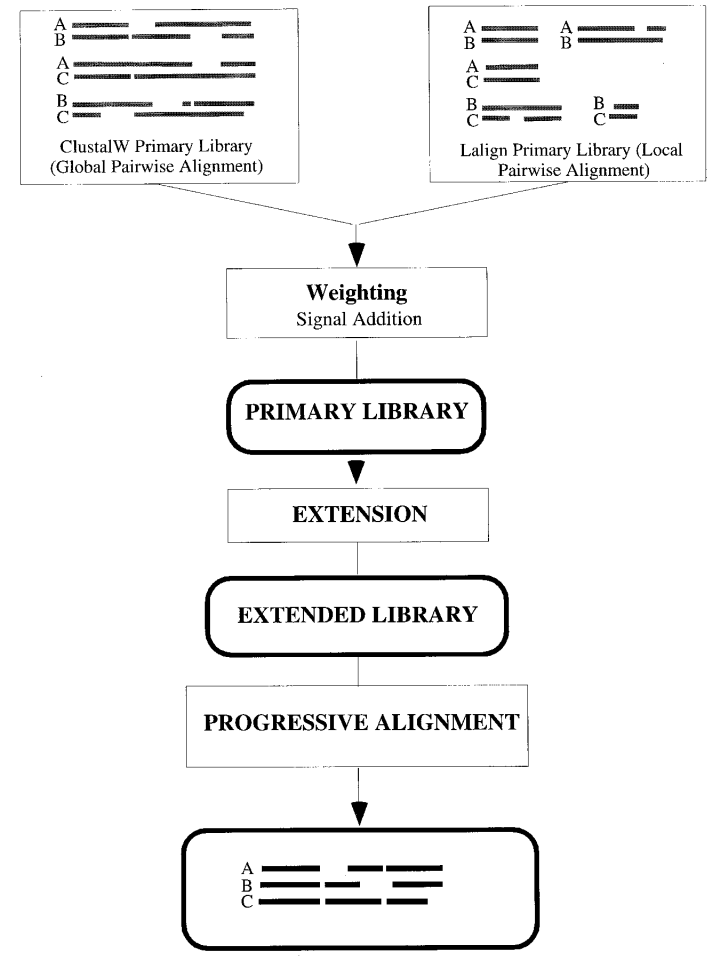
\includegraphics[width=0.5\linewidth]{1.png}
\caption{Layout of the T-Coffee strategy; the main steps required to compute a multiple sequence alignment using the T-Coffee method. Square blocks designate procedures while rounded blocks indicate data structures.}
\label{fig:structure}
\end{figure}

\section{T-Coffee Algorithm}
T-Coffee (Tree-based Consistency Objective Function for alignment Evaluation) has two main features.
\\
First, it provides a simple and flexible means of generating multiple alignments, using heterogeneous data sources. The data from these sources are provided to T-Coffee via a \textbf{library} of pair-wise alignments.
\\
The main feature of T-Coffee is the \textbf{optimization} method, which is used to find the multiple alignment that best fits the pair-wise alignments in the input library.
A so-called \textbf{progressive strategy} is implemented, which is similar to that used in ClustalW. The difference from CustalW is that T-Coffe makes use of the information in the library to carry out progressive alignment in a manner that allows us to consider the alignments between all the pairs while we carry out each step of the progressive multiple alignment.
This gives us progressive alignment, with all its advantages of speed and simplicity, but with a far lesser tendency to make errors like the one shown in Figure \ref{fig:2}(a), i.e. misalignment of the word CAT.
T-Coffee is a progressive alignment with an ability to consider information from all of the sequences during each alignment step, not just those being aligned at that stage.

\begin{figure}[H]
\centering
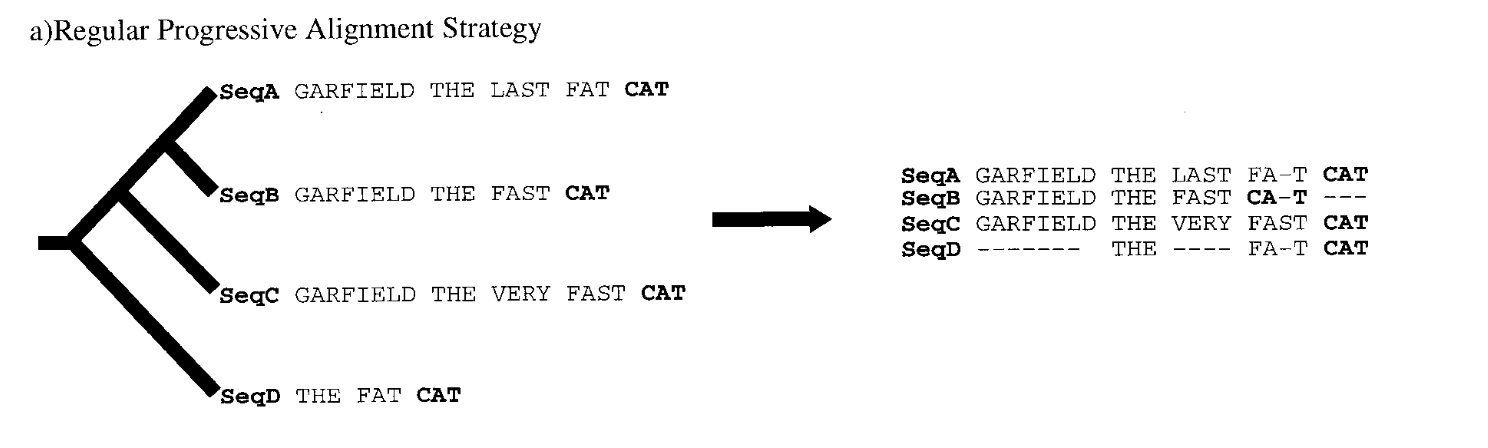
\includegraphics[width=0.8\linewidth]{2a.png}
c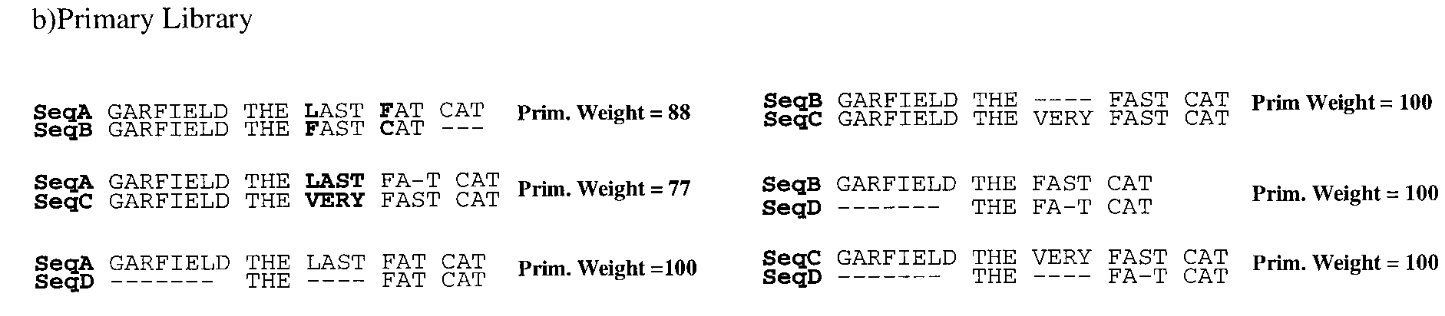
\includegraphics[width=0.8\linewidth]{2b.png}
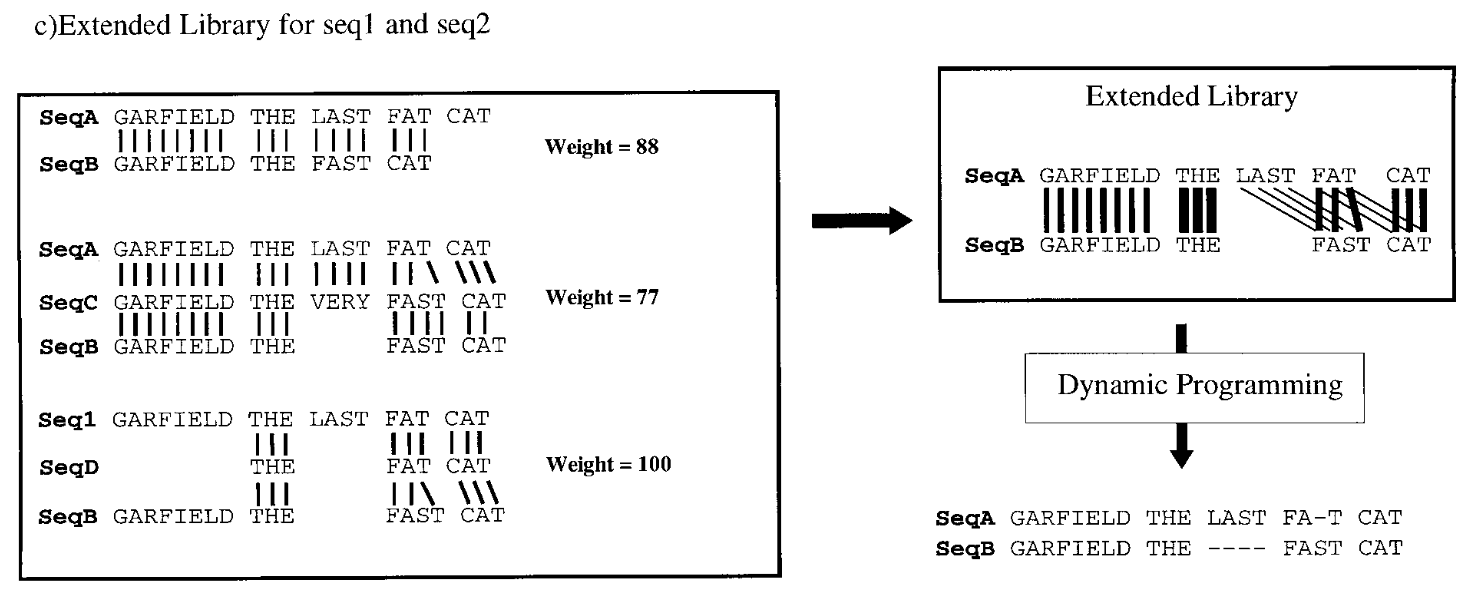
\includegraphics[width=0.8\linewidth]{2c.png}
\caption{The library extension. \textbf{(a) Progressive alignment}. Four sequences have been designed. The tree indicates the order in which the sequences are aligned when using a progressive method such as ClustalW. The resulting alignment is shown, with the word CAT misaligned. \textbf{(b) Primary library}. Each pair of sequences is aligned using ClustalW. In these alignments, each pair of aligned residues is associated with a weight equal to the average identity among matched residues within the complete alignment (mismatches are indicated in bold type). \textbf{(c) Library extension for a pair of sequences}. The three possible alignments of sequence A and B are shown (A and B, A and B through C, A and B through D). These alignments are combined, as explained in the text, to produce the position-specific library. This library is resolved by dynamic programming to give the correct alignment. The thickness of the lines indicates the strength of the weight.}
\label{fig:2}
\end{figure}


\subsection{Generating a primary library of alignments}
The primary library contains a set of pair-wise alignments between all of the sequences to be aligned.
In the library, we include information on each of the $N(N - 1)/2$ sequence pairs, where $N$ is the number of sequences. Here, we use two alignment sources for each pair of sequences, one \textbf{local} and one \textbf{global}.
The global alignments (Figures \ref{fig:structure} and \ref{fig:2}(b)) are constructed using ClustalW on the sequences, two at a time. The local alignments (Figure \ref{fig:structure}) are the ten top scoring non-intersecting local alignments, between each pair of sequences, gathered using the Lalign program.
\\
In the library, each alignment is represented as a list of pair-wise residue matches (e.g. residue x of sequence A is aligned with residue y of sequence B).
In effect, each of these pairs is a constraint.
All of these constraints are not equally important. Some may come from parts of alignments that are more likely to be correct. This is taken into account when computing the multiple alignment and give priority to the most reliable residue pairs. This is achieved by using a weighting scheme, which is described in subsection \ref{sub:weights}.

\subsection{Derivation of the primary library weights} \label{sub:weights}
T-Coffee assigns a weight to each pair of aligned residues in the library (Figure 2(b)).
The \textbf{sequence identity} weighting scheme is used, which has been prove to be effective and of great simplicity.
Libraries are lists of weighted pair-wise constraints. Each constraint receives a weight equal to percent identity within the pair-wise alignment it comes from (Figure \ref{fig:2}(b)).
For each set of sequences, two primary libraries are computed along with their weights, one using ClustalW (global alignments; Figure \ref{fig:2}(b)) and the second using Lalign (local).

\subsection{Combination of the libraries}
The aim is the efficient combination of local and global alignment information.
This is achieved by pooling the global and local primary libraries in a simple process of \textbf{addition}.
If any pair is duplicated between the two libraries, it is merged into a single entry that has a weight equal to the sum of the two weights.
Otherwise, a new entry is created for the pair being considered (process called unofficially "\textbf{stacking" of the signal}).
Pairs of residues that did not occur are not represented (weight of zero).
\\
This primary library can be used directly to compute a multiple sequence alignment.
However, we enormously increase the value of the information in the library by examining the consistency of each pair of residues with residue pairs from all of the other alignments.
For each pair of aligned residues in the library, we can assign a weight that reflects the degree to which those residues align consistently with residues from all the other sequences.
This process is called library extension (subsection \ref{sub:extension}).

\subsection{Extending the library} \label{sub:extension}
Fitting a set of weighted constraints into a multiple alignment is a well known NP-complete problem.
\\
We circumvent the problem by using a heuristic algorithm that we call \textbf{library extension} (Figure \ref{fig:2}(c)). The idea is to combine information in such a manner that the final weight, for any pair of residues, reflects some of the information contained in the whole library. To do so, a \textbf{triplet approach} is used, as summarized in Figure \ref{fig:2}(c).
\\
It is based on taking each aligned residue pair from the library and checking the alignment of the two residues with residues from the remaining sequences.
\subsubsection{A quick example}
For instance, let us consider the four sequences A, B, C
and D of Figure 2. Let us call A(G) the G of GARFIELD in sequence A, B(G) the equivalent G in sequence B and W(A(G), B(G)) the weight associated with this pair of symbols in the primary library. In the direct alignment of A and B, A(G) and B(G) are matched (Figure \ref{fig:2}(b) and (c)). Therefore, the initial weight for that pair of residues can be set to 88 (primary weight of the alignment of sequence A and B, which is the percent of identity of this pair). If we now look at the alignment of sequence A and sequence B through sequence C (Figure \ref{fig:2}(c)), we can see that the A(G) and C(G) are aligned, as well as C(G) and A(G). We conclude that there is an alignment of A(G) with B(G) through sequence C. We associate that alignment with a weight equal to the minimum of $W_1 = W(A(G), C(G))$ and $W_2 = W(C(G), B(G))$. Since $W_1 = 77$ and $W_2 = 100$, the resulting weight is set to 77. In the extended library, this new value is added to the previous one to give a total weight of 165 for the pair A(G), B(G). The complete extension will require an examination of all the remaining triplets. Not all of them bring information. For instance, the alignment of A and B through sequence D does not contain any information relative to A(G) or B(G), and, therefore, it has no influence on the weight associated with A(G) and B(G). In summary, the weight associated with a pair of residues will be the sum of all the weights gathered through the examination of all the triplets involving that pair.

\subsubsection{Alignment}
Weights will be zero for any residue pairs that never occur (this will be true of the majority of residue pairs). Otherwise, the weight will reflect a
combination of the similarity of the pair of sequences or sequence segments that the residue pair comes from and the consistency of that residue pair with all other residue pairs in the primary library. These scores can then be used to align any two sequences from our data set using conventional dynamic programming.
When one normally aligns a pair of sequences, one uses a set of scores derived from some general table of amino acid weights such as a Blosum matrix. In our case, we can replace that matrix with a set of scores that are specific to every possible pair of residues in our two sequences.
This will allow an alignment to be carried out that will take account of the particular residues in the two sequences but will also be guided towards consistency with all of the other sequences in the data set.

\subsection{Progressive alignment strategy}
The \textit{normal} progressive alignment strategy consists in creating a guide tree (a phylogenetic tree) using the neighbor-joining method.
The closest two sequences on the tree are aligned first using normal dynamic programming.
This pair of sequences is then fixed and any gaps that have been introduced cannot be shifted later. Then the next closest two sequences are aligned or a sequence is added to the existing alignment of the first two sequences, depending which is suggested by the guide tree.

As used here, the procedure does not require any additional parameters such as gap penalties. This stems, in part, from the fact that the substitution values (the library weights) were computed on alignments where such penalties had already been applied. Furthermore, high scoring segments that show consistency within the data set see their score enhanced by the extension to such a point that they become insensitive to gap penalties.

\section{Biological validation}
\textit{I chose not to report the comparisons with other tools and the complexity of the algorithm. If needed, exhaustive tabled can be found in the paper.}

\subsection{Application to serine/threonine kinases}
A major application of any alignment algorithm will be the delineation of motifs or domains.
19 sequences from a sub-family of the serine/threonine kinases were provided. Each sequence in the alignment contains a nucleotide-binding site (NBS).
In all these sequences, the NBS is followed by a second conserved motif toward the C terminus.
T-Coffee was able to accurately align 18 of the 19 NBSs, ClustalW was only able to correctly align 16 of these NBSs. The second motif is more difficult
because of the long indel in st11 yeast. Here as well, T-Coffee can properly align 18 of the motifs, while ClustalW get 15 correct.
As a result of combining local and global alignment information, T-Coffee managed to align almost all of the motifs as in the BaliBase reference alignment. Moreover, T-Coffee was the only program that correctly aligned the second motif of kp68 human, which is an interferon-induced kinase.

\chapter{Protein profiles with HMMs}

\graphicspath{{chapters/13/}}
\chapter{Construction of phylogenetic trees}
\emph{A method based on \textbf{mutation distances} as estimated from cytochrome \textit{c} sequences is of general applicability (1967)}

\section{What are phylogenetic trees}
They are graphs made up of nodes, which represent the taxonomic units and from branches that join the nodes, representing the distances between the two.
\\
Topology is defined as the general structure of a tree. If to the branches evolutionary distance is not given, we have a cladogram (I), otherwise we have a filogram (II) and with time a dendogram (III).
\\
Trees without root do not foresee evolutionary meanings in time terms and describe simply the relationships between sequences. Trees with root they accept the hypothesis as true of the molecular clock and the nodes they are in a specific
temporal order.
\begin{figure}[H]
		\centering
		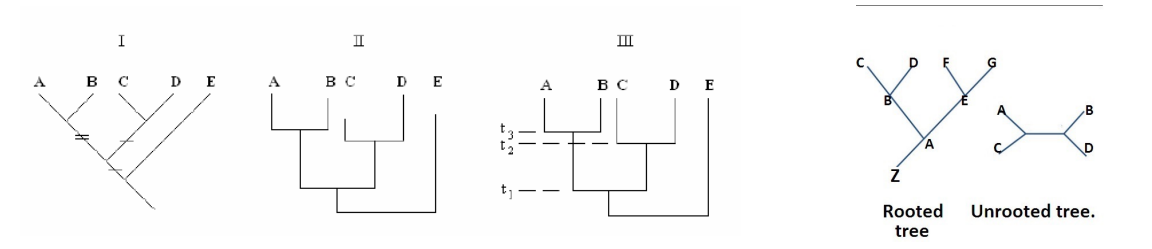
\includegraphics[width=0.9\textwidth]{grams.png}
		\caption{Topologies of phylogenetic trees}
		\label{fig:1}
	\end{figure}

\section{Introduction}
Some methods to constructs phylogenetic trees were developed before the one that will be discussed here, like studies of the degree of interspecific hybridization of DNA, number of amino acid replacements between homologous proteins, etc.
These methods are not satisfactory, because:
\begin{itemize}
\item i) the portion of the genome examined was often very resticted
\item ii) Low accuracy in the mutation distance between the genes examined
\item iii) no adequate mathematical treatment of large datasets
\end{itemize}

To tackle especially points ii) and iii), a new method is hereby proposed and the validity of the results is carried out with the construction of a tree considering only cytochrome \textit{c}, for much much information is available.
Even just considering one gene, the resulting tree is much similar to the phylogenetic tree constructed directly from biological data.

\subsection{Ancenstral genes, Orthologs and Paralogs}
Among homologous genes, one has to distinguish \textbf{orthologous} from \textbf{paralogous} sequences. Orthologs are \textbf{homologous} genes in different species that diverged from a single \textbf{ancestral gene} after a speciation event and paralogs are homologous genes that originate from the intragenomic duplication of an ancestral gene.

\subsection{Proteins or nucleic acids?}
For molecular phylogeny it is preferable to use nucleotide sequences.
In phylogeny both are used, but it is necessary to fix some key aspects that define the different action ranges of the two:
\begin{itemize}
\item Protein sequences
	\begin{itemize}
	\item need 20x20 replacement matrices, very complex to deal with
	\item are the expression of coding regions only
	\item identical amino acids can be the expression of multiple codons
	\end{itemize}

\item Nucleotide sequences
	\begin{itemize}
	\item they can be described with 4x4 matrices.
	\item can be extracted from non-coding genomic sequences, therefore with higher variation
	\item they have no degeneration or redundancy.
\end{itemize}

\end{itemize}

\section{Determining the mutation distance}
The mutation distance between two cytochromes is defined here as the minimal number of nucleotides that would need to be altered in order for one cytochrome to code for the other. This distance is determined by making pair wise comparison of homologous amino acids. For each pair a mutation value is taken from a pre-defined table, which gives the minimum number of nucleotide changes required to convert the coding from one amino acid to the other. 
\\
For each possible pairing of cytochromes, the 110 mutation values found are summed to obtain the minimal mutation distance. 
The basic approach tot he construction of the tree is illustrated in figure \ref{fig:1}, which shows three hypothetical proteins, A, B and C, and their mutation distances. There are two fundamental problems: 

\begin{itemize}
\item Which pair to join first? As a first approximation, one solves it by simply choosing the pair with the smallest mutation distance, which in this case is A and B, with a distance of 24. A and B are shown connected at the lower apex. 
\item What are the lengths of legs \textit{a, b} and \textit{c}? One notes that the distance from A to C, 28, is 4 less than the distance form B to C. Meaning, there must have bee at least 4 countable mutations in the descent of B from the lower apex than in the descent of A.
\end{itemize}

\begin{figure}[H]
		\centering
		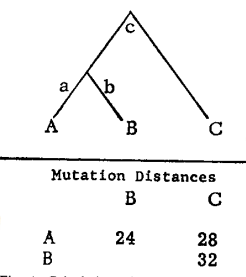
\includegraphics[width=0.4\textwidth]{1.png}
		\caption{Calculation of observed mutation distances. The upper apex represents a hypothetical ancestral organism that divided into two descending lines, one of which subsequently also divided. Thus we have three present-day species, A, B, C. The number of observable mutations that have occurred since the A and B lines of descent diverged are represented respectively by \textit{a} end \textit{b}. The number of mutations that separate the lower apex and C is represented by \textit{c}. The sums of $a+b, a+c, b+c$ then are the mutation distances of the three species as currently observed.}
		\label{fig:1}
	\end{figure}


When information from more than three protein is utilized, the basic procedure is the same, except that initially each protein is assigned to its own subset. One then simply joins two subsets to create a single, more comprehensive subset, and the process is repeated until all proteins are members of  a single subset. 
A phylogenetic tree is but a grphical representaion of the order in which the subsets were joined. 
\\
In the case of this study, they started with 20 subsets, each subset consisting of a single cytochrome \textit{c} amino acid sequence. One arbitrarily accepts, from among all the possible pairings examined, that assigned of protein subsets to sets A, B and C which provides the lowest average mutation distance from A to B. The leg lengths are then recorded. Henceforth the proteins of A and B so joined are treated as a single subset, and the entire procedure described in the preceding paragraph is repeated.  Thus the number of proteins($N$) is reduced by 1 at each cycle. The tree will be produced after $N-1$ joinings. 

\subsection{Genetic distances}
\emph{From slides, lec 13}
\\
For the phylogenetic distinction of two sequences, it is necessary to know how much they diverge. We therefore need an objective parameter and a calculable, defined genetic distance. 
For conserved nucleic acids, the number of percentage substitutions observed after multiple alignments

\begin{equation}
d = \frac{n. replacements}{length}
\end{equation}

For less conserved nucleic acids the \textit{d} is corrected with the Jukes-Cantor formula:

\begin{equation}
d'= -\frac{3}{4}log(1- \frac{4}{3} d)
\end{equation}

For proteins, aligned with a replacement matrix, it is often used the approximated formula:

\begin{equation}
d =  \frac{(Sobs - Srand)}{(Smax -Srand}
\end{equation}

With Sobs the score of the alignment, Smax average of the scores of the alignments of all proteins with themselves, Srand score expected for sequences of the same length and composition. 

\section{Testing alternative trees}
Because of the arbitrary nature of the rule by which proteins were assigned to sets A and B, the initial tree will not necessarily represent the best use of the information. The solution provided by the authors is simply to construct another tree by assigning an alternative pair of protein subsets to sets A and B whenever the mutation distance between the two subsets is not greater by some arbitrary amount than that between the members of the initial pair used in constructing the initial phylogenetic tree. 

\subsection{Standard deviation}
If the absolute difference between two such mutation distances $|(i,j)-(j,i)|$ is multiplied by $100$ and divided by (i,j), the result is the  of change from the input data. If such values are squared and the squares are summed over all values of $i < j$, the resultant sum ($\mathcal{E}$) may be used to obtain the percent "standard deviation" of the reconstructed values from the input mutation distances. The number of mutation distances summed is $N(N-1)/2$. The number is reduced by 1, divided into the sum $\mathcal{E}$ and the square root taken, the result is the percent "standard deviation". 

\section{The statistically optimal tree}
In testing phylogenetic alternatives, one is seeking to minimize the percent standard deviation.
\\
In addition to using a single gene product to discover evolutionary relationships among several species, one can similarly delineate evolutionary relationships among different genes (int he paper the gene phylogeny, from the amino acid sequence was reconstructed for human alpha, beta, gamma and delta hemoglobinn chains and whale myoglobin).
\\
A cautionary note may be derived from this. A wildly incorrect result could e easily be obtained if the presence of multiple, homologous genes were not recognized and a phylogeny were reconstructed from sequences which were coded for, say, half by genes for alpha hemoglobin chains and half by genes for beta hemoglobin chains. This results from the speciation having occurred more recently than the gene duplication which permitted the separate evolution of the alpha and beta genes.

\section{Phylogenetic relationships in trees}
\emph{From slides, lec 13}
\\ 
The systems for building trees aims to discover how the sequences are in
relation to each other: the data (the sequences themselves or distances) are used to create a system of equations that models "when" the sequences diverge (the nodes) and how extensive it is the separation separation (branches).

It starts from a theoretical tree in which the various OTUs are inserted, without giving importance to the various branches. The goal is to understand how, how much and where they fork using various criteria, not necessarily molecular.

\subsection{Fitch-Margoliash algorithm (FM)}
\begin{figure}[H]
		\centering
		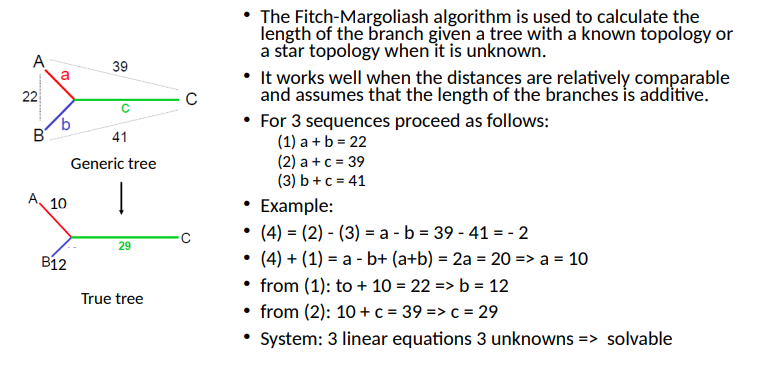
\includegraphics[width=0.8\textwidth]{ex1.png}
		\caption{}
		\label{fig:ex1}
	\end{figure}

















\chapter{Toward defining the course of evolution: minimum change for a specific tree topology} 

\chapter{Evolutionary Trees from DNA Sequences: A Maximum Likelihood Approach}



\end{document}
